%!TEX root=../document.tex

\section{Ergebnisse}
\label{sec:Ergebnisse}

\subsection{Installation von OpenLDAP}
(Geschrieben von Kevin Waldock)

\subsubsection{Vorbereitungen}
Bevor OpenLDAP installiert wird, muss zunächst ein Domain-Name bzw ein eigener hostname eingerichtet werden. Wird dies nicht gemacht, so wird OpenLDAP für den Admin den DN ``cn=admin,dc=nodomain,dc=org'' verwenden.

Um nun die Hosts-Datei zu editieren öffnet man zunächst die Linux-Konsole (Terminal). Um die Hosts-Datei zu editieren muss man ein Editor starten zu der Datei /etc/hosts. Man benötigt Admin-Rechte um die Datei zu editieren. Ich habe den Editor gedit ausgewählt.

\verb|sudo gedit /etc/hosts|

Ich hab die Zeile mit dem Hostname für 127.0.1.1 editiert und meinen eigenen hinzugefügt. Ich habe mich für den Hostname ``waldock'' und die Domain "waldock.4chit.at" entschieden. Nach dem Editieren der Datei sollte es nun so aussehen:

\begin{center}
	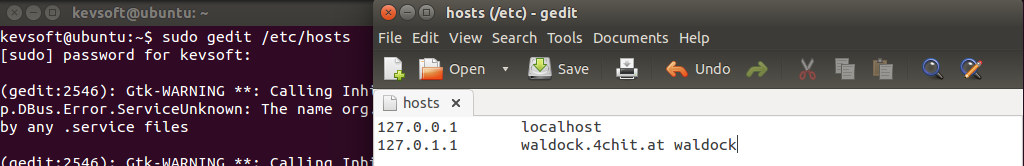
\includegraphics[width=1.0\linewidth]{images/a1_hostsfile.PNG}
\end{center}

Jedoch reicht dies noch nicht aus. Zusätzlich muss die Hostname-Datei ebenfalls editiert werden. Dazu wird ebenfalls gedit aufgerufen:

\verb|sudo gedit /etc/hostname|

Diese Datei beinhaltet den hostname des Betriebsystems. Da ersetzen wir den aktuellen Hostname mit ``waldock''.

Danach muss nur noch ein Neustart durchgeführt werden und der Hostname ist richtig konfiguriert.

